\documentclass[10pt,twocolumn,letterpaper]{article}
\usepackage{cvpr}
\usepackage{times}
\usepackage{graphicx}
\usepackage{amsmath,amssymb}
\usepackage{booktabs}
\usepackage{listings}
\usepackage[pagebackref,breaklinks,colorlinks,bookmarks=false]{hyperref}
\def\confName{CVPR}
\def\confYear{2022}

\lstset{language=Python,basicstyle=\ttfamily\scriptsize,breaklines=true,
  numbers=left,numberstyle=\tiny,columns=fullflexible,showstringspaces=false,
  literate={×}{{$\times$}}1 {α}{{$\alpha$}}1 {–}{{--}}1 {…}{{\ldots}}1}
\newcommand{\codefile}[1]{\lstinputlisting[title=\lstname]{#1}}

\begin{document}
\title{Adaptive Eulerian Video Magnification with Local Frequency Selection and Edge-Preserving Filtering}
\author{Pradeep Bishnoi\\
240756\\
{\tt\small pradeep24@iitk.ac.in}
\and
Manthan J\\
IIT Kanpur\\
\and
Mayank Verma\\
IIT Kanpur\\
\and
Harsh Ramteke\\
IIT Kanpur\\
}


\maketitle

\begin{abstract}
Eulerian video magnification can reveal small periodic motions, but a fixed
temporal passband can miss the target and whole-frame amplification can
accentuate unrelated changes. We combine a local Welch spectrum, a feathered
magnification region, and optional bilateral filtering of signed pyramid
details in a CPU implementation. The estimator recovers the 1.2\,Hz motion of
a synthetic edge and selects 0.9\,Hz in a wrist clip despite a larger
out-of-band peak at 0.1\,Hz. The spatial gate eliminates changes outside the
selected rectangle before video encoding. Matched ablations quantify the
change in target response, synthetic reference error, and processing cost.
\end{abstract}

\section{Introduction}
Eulerian video magnification (EVM) operates on temporal intensity variations
at fixed image locations. Wu et al.~\cite{wu2012eulerian} showed how spatial
decomposition and bandpass filtering reveal weak motion and color variations.
An offline implementation can use forward--backward filtering to avoid
temporal phase lag. For a localized periodic event, spatial selection also
avoids amplifying motion elsewhere in the frame.

We combine an ROI-based frequency estimate, localized luminance
magnification, and a per-level bilateral filter. The interface displays both
the full spectrum and the restricted search range so that the selected
frequency can be checked against visible spectral peaks.

\section{Related Work}
Liu et al.~\cite{liu2005motion} estimate motion trajectories and re-render the
scene. Eulerian methods instead amplify local image variations directly.
The linear approach of Wu et al.~\cite{wu2012eulerian} uses a spatial pyramid,
while Wadhwa et al.~\cite{wadhwa2013phase} magnify local phase changes.
Remote photoplethysmography also extracts periodic signals from
video~\cite{verkruysse2008remote,poh2010noncontact}. Here the spectral estimate
sets a filter band for visualization. Its cycles-per-minute value describes
the selected oscillation.

\section{Method}
\subsection{Spatial and Temporal Baseline}
For small translation $\delta(t)$, a local intensity profile satisfies
\begin{equation}
  I(x,t) \simeq f(x) + \delta(t) f'(x).
\end{equation}
If the bandpass isolates $\delta(t)f'(x)$, adding $\alpha$ times that term
approximates a shift of $(1+\alpha)\delta(t)$. Large displacements and gain
can violate the first-order approximation.

The input BGR frames are converted to luminance and decomposed into three
signed Laplacian detail bands~\cite{burt1983laplacian}. The Gaussian base is
omitted from the adjustment to target spatial detail. Each coefficient
trace is filtered by a fifth-order Butterworth bandpass in second-order
sections, applied forward and backward. The detail residual is reconstructed,
scaled, and added equally to each original channel. Clipping the shared
adjustment to the available channel headroom preserves channel differences.

\subsection{Frequency Selection}
For a detection rectangle $R_d$, let $s_t$ be the mean green intensity.
The pipeline removes a linear trend and estimates power $P(f)$ by Welch
averaging~\cite{welch1967use} with Hann windows and 50\% overlap. The segment
duration targets the maximum of ten seconds, three periods at the lower
search bound, and five frequency steps across the search band, capped by
clip duration. Local peaks in the search band are ranked by prominence.
The default range is 0.65--3.00\,Hz, with the upper edge limited by the
sampling rate. The confidence heuristic is
\begin{equation}
  C = \frac{P(f^\star)}
  {\max\!\big(\operatorname{median}_{f \in \mathcal B} P(f),\epsilon\big)},
\end{equation}
where $\mathcal B$ is the set of eligible bins and $\epsilon$ is a numerical
floor. A usable peak defines a passband extending 0.20\,Hz on either side,
bounded by the search range and Nyquist margin. If the estimator rejects
the signal, the app uses the manual band.

\subsection{Localization and Artifact Suppression}
Automatic ROI mode ranks periodic image tiles after removing the shared
median tile trace. It can estimate frequency on a compact patch and
magnify a larger box centered on that patch. Manual ROI mode uses the
selected box for both operations. The filter applies the rectangle
support at each scale using a Gaussian pyramid of the binary mask.
The reconstructed adjustment is gated by an inward linear feather of
at most eight pixels, which prevents coarse levels from changing pixels
outside the selected rectangle.

The optional bilateral filter~\cite{tomasi1998bilateral} averages nearby
coefficients with similar values in each filtered detail band. We apply it
before reconstruction with a five-pixel neighborhood diameter, spatial
$\sigma_s=5$, and range $\sigma_r=25.5/\alpha$ in pre-gain intensity units
for the tested positive gain. This makes the range parameter correspond
to a constant tolerance in amplified intensity units. Signed details are
retained throughout reconstruction.

\section{Experiments}
\subsection{Protocol}
The deterministic synthetic clip contains a noisy edge with a
0.24-pixel sinusoidal displacement at 1.2\,Hz and a separate 0.8\,Hz
distractor. The clean reference uses the same edge with displacement
scaled by $1+\alpha$. The real inputs are the MIT wrist clip at half
resolution and the baby and guitar clips bundled with PyEVM. All runs
use $\alpha=4$ and the same decoded frames across configurations.
The benchmark scales clips to a maximum side of 320 pixels.

The baseline uses the manual band over the full frame. We also test each
feature individually, automatic band plus ROI, and the full pipeline.
The last two rows isolate the bilateral toggle at fixed ROI and band.
We measure RMS output--input change outside the ROI before encoding
and the ratio of output to input sinusoidal amplitude at the target
frequency in the detection patch. On the synthetic clip, we also
measure RMSE against the clean reference in the interior of the ROI,
excluding one second at each endpoint. Real clips provide no clean
magnified reference. Runtime includes the spectral estimate for automatic
configurations and excludes decoding, plotting, and video encoding.
Effective FPS is the number of processed frames divided by this runtime.

\begin{table}[t]
\centering\small
\setlength{\tabcolsep}{3pt}
\begin{tabular}{@{}lrrrr@{}}
\toprule
Wrist & Outside RMS & Gain & s & FPS\\
\midrule
Baseline & 2.12 & 2.41 & 13.36 & 66.9 \\
Auto band only & 2.12 & 2.41 & 12.25 & 73.0 \\
ROI only & 0.00 & 2.41 & 11.16 & 80.1 \\
Bilateral only & 0.63 & 2.30 & 12.68 & 70.5 \\
Auto band + ROI & 0.00 & 2.41 & 10.97 & 81.5 \\
Full pipeline & 0.00 & 2.30 & 11.66 & 76.7 \\

\bottomrule
\end{tabular}
\caption{Matched wrist results on 894 frames at $320 \times 176$ and
30 source FPS. RMS is measured in 8-bit intensity levels. Gain is measured
at the selected 0.9\,Hz frequency.}
\label{tab:wrist}
\end{table}

\begin{table}[t]
\centering\small
\setlength{\tabcolsep}{3pt}
\begin{tabular}{@{}lrrrr@{}}
\toprule
Synthetic & RMSE & Gain & s & FPS\\
\midrule
Baseline & 9.67 & 1.02 & 1.44 & 249.4 \\
Auto band only & 4.93 & 1.45 & 1.39 & 259.0 \\
ROI only & 9.67 & 1.04 & 1.14 & 315.7 \\
Bilateral only & 9.74 & 1.03 & 1.37 & 262.4 \\
Auto band + ROI & 4.93 & 1.79 & 1.04 & 347.7 \\
Full pipeline & 6.45 & 1.66 & 1.14 & 315.5 \\

\bottomrule
\end{tabular}
\caption{Matched synthetic results on 360 frames at $160 \times 80$ and
30 source FPS. RMSE is in 8-bit intensity levels. Gain is measured at the
known 1.2\,Hz target frequency.}
\label{tab:synthetic}
\end{table}

\subsection{Results}
The wrist detection patch is $(192,100,18,18)$ and the larger
magnification box is $(174,82,54,54)$ in $(x,y,w,h)$ coordinates.
Figure~\ref{fig:psd} explains why the 0.9\,Hz peak sets the filter:
the taller 0.1\,Hz component lies outside the search range. The manual
wrist band and the estimated band both span 0.70--1.10\,Hz. On that clip,
the automatic mode reproduces the hand-tuned band. The synthetic case
uses a manual band that omits the target frequency to test the behavior
when the initial band is wrong.

\begin{figure}[t]
\centering
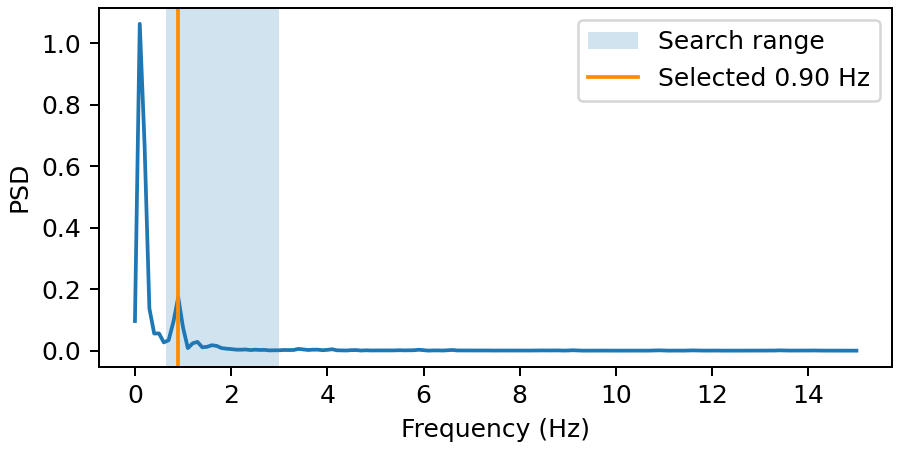
\includegraphics[width=\linewidth]{results/validation/wrist-psd.png}
\caption{Full wrist ROI spectrum with the eligible search range shaded.}
\label{fig:psd}
\end{figure}

\begin{figure*}[t]
\centering
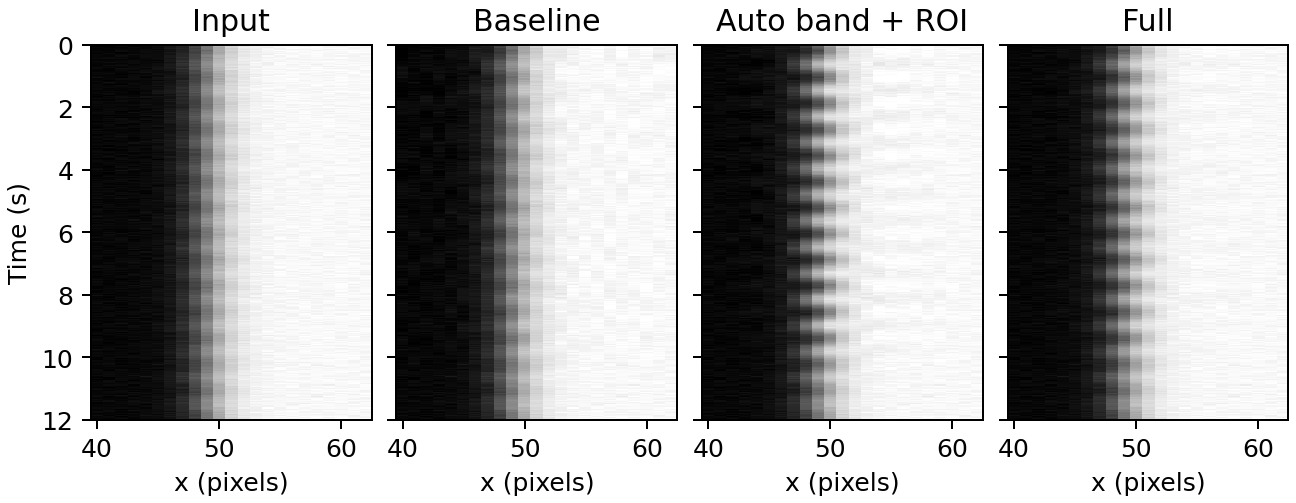
\includegraphics[width=0.73\textwidth]{results/validation/synthetic-xt.png}
\caption{Synthetic space--time slices through the same horizontal scan
line. The columns use a common grayscale range.}
\label{fig:xt}
\end{figure*}

Tables~\ref{tab:wrist} and~\ref{tab:synthetic} summarize the matched
comparisons. On the wrist, localization reduced outside-region RMS
from 2.12 intensity levels to zero. At the same ROI and band, bilateral
filtering reduced the wrist tone gain from 2.41 to 2.30.
On the synthetic clip, choosing the correct band with ROI reduced clean
reference RMSE from 9.67 to 4.93 levels. Enabling bilateral filtering
raised RMSE to 6.45 and reduced tone gain from 1.79 to 1.66.
These settings attenuate useful motion along with other variation.
The full wrist configuration processed 76.7 frames per second in one
CPU run, excluding I/O. Timing differences between individual rows
include run-to-run variability.

The CSV also records baby and guitar runs, and the benchmark exports
an aligned space--time slice for each clip. A local phone wrist excerpt
yielded 1.60\,Hz (about 96 cycles/min), compared with a user-reported
88 beats/min. The reference was not synchronized to the excerpt.
Aliasing, camera motion, and ROI placement can change the interpretation
of peaks on real video. A throat recording was unavailable for evaluation.

\section{Conclusion}
The integrated pipeline uses spatial and spectral selection to target
small oscillations. The synthetic reference makes it possible to measure
the tradeoff between visual smoothing and motion retention. On real
clips the spectrum, background leakage, and timing provide reproducible
diagnostics, while a synchronized physiological or motion reference
would be needed to validate the identity of the detected oscillation.

{\small
\begin{thebibliography}{99}

\bibitem{wu2012eulerian}
H.-Y. Wu, M. Rubinstein, E. Shih, J. Guttag, F. Durand, and W. T. Freeman.
\newblock Eulerian video magnification for revealing subtle changes in the world.
\newblock {\em ACM Transactions on Graphics}, 31(4):65, 2012.

\bibitem{wadhwa2013phase}
N. Wadhwa, M. Rubinstein, F. Durand, and W. T. Freeman.
\newblock Phase-based video motion processing.
\newblock {\em ACM Transactions on Graphics}, 32(4):80, 2013.

\bibitem{liu2005motion}
C. Liu, A. Torralba, W. T. Freeman, F. Durand, and E. H. Adelson.
\newblock Motion magnification.
\newblock {\em ACM Transactions on Graphics}, 24(3):519--526, 2005.

\bibitem{poh2010noncontact}
M.-Z. Poh, D. J. McDuff, and R. W. Picard.
\newblock Non-contact, automated cardiac pulse measurements using video imaging and blind source separation.
\newblock {\em Optics Express}, 18(10):10762--10774, 2010.

\bibitem{verkruysse2008remote}
W. Verkruysse, L. O. Svaasand, and J. S. Nelson.
\newblock Remote plethysmographic imaging using ambient light.
\newblock {\em Optics Express}, 16(26):21434--21445, 2008.

\bibitem{burt1983laplacian}
P. J. Burt and E. H. Adelson.
\newblock The Laplacian pyramid as a compact image code.
\newblock {\em IEEE Transactions on Communications}, 31(4):532--540, 1983.

\bibitem{welch1967use}
P. D. Welch.
\newblock The use of fast Fourier transform for the estimation of power spectra: a method based on time averaging over short, modified periodograms.
\newblock {\em IEEE Transactions on Audio and Electroacoustics}, 15(2):70--73, 1967.

\bibitem{tomasi1998bilateral}
C. Tomasi and R. Manduchi.
\newblock Bilateral filtering for gray and color images.
\newblock In {\em Proc.\ IEEE International Conference on Computer Vision (ICCV)}, pages 839--846, 1998.

\end{thebibliography}
}

%%%%%%%%% APPENDIX
\clearpage

\appendix
\section{Reproduction}
The source is available at
\url{https://github.com/Manthan-J/EE604-Motion-Magnification}.
Run \texttt{python benchmark\_evm.py} from the repository root to regenerate
the tables, CSV and figures. Use \texttt{python -m streamlit run app2.py}
to launch the demonstration. The benchmark also accepts a local video
and explicit ROI for additional recordings. See the repository README
for dependencies and commands.

\section{Source Code}
\codefile{src/spatial.py}
\codefile{auto_frequency.py}
\codefile{auto_roi.py}
\codefile{roi_magnification.py}
\codefile{app2.py}
\codefile{benchmark_evm.py}
\end{document}
